% MAS1004 Assignment 1: four-class long report. Compile with XeLaTeX.
\documentclass[11pt]{article}
\usepackage{mas1004}
\reporttitle{Assignment 1: Classifying Korean album covers by release era}
\studentname{Your name}
\studentid{Your student ID}
\newcommand{\resultfigure}[2]{\begin{center}\picturefile{#1}\captionof{figure}{#2}\end{center}}
\begin{document}
\makeheader

\section*{Problem 1. Categories and images}
\subsection*{Why these categories}
I chose Korean album covers from four eras: the 1980s--1990s, 2000s, 2010s, and 2020s. I enjoy music and am interested in cultural and social change, so I wanted to see whether cover designs distinguish release eras. I combined the 1980s and 1990s because I expected limited data for the 1980s and possibly similar visual styles.

\subsection*{What I expected the model to use}
Before training, I expected colour, resolution and scan traces, typography, layout, and photographic or graphic styles to provide clues. I was concerned that the model might rely on superficial correlations such as low image quality rather than meaningful era-related design.

\subsection*{Images per category}
\begin{center}
\begin{tabular}{lrrr}\toprule
Era & Initial dataset & Final CLEAN dataset & New images\\\midrule
1980s--1990s &146&93&8\\
2000s &144&79&6\\
2010s &167&87&8\\
2020s &175&114&5\\\midrule
Total &632&373&27\\\bottomrule
\end{tabular}
\captionof{table}{Readable images before splitting, and images from a new source.}
\end{center}
The initial runs used 506 training and 126 test images; CLEAN used 298 training and 75 test images. The class folders, in table order, are:
\begin{itemize}
\item \path{1980s_1990s_korean_album_covers}
\item \path{2000s_korean_album_covers}
\item \path{2010s_korean_album_covers}
\item \path{2020s_korean_album_covers}
\end{itemize}

\section*{Problem 2. Preparing an image}
\texttt{prepare\_image()} converts to RGB, resizes the shorter side to 256 using bilinear interpolation, takes the central $224\times224$ crop, divides pixels by 255, and normalizes with RGB means $(0.485,0.456,0.406)$ and standard deviations $(0.229,0.224,0.225)$. It returns a \texttt{float32} array of shape $(3,224,224)$.

\resultfigure{figures/P2_preprocessing.png}{Original cover (left) and resized, centre-cropped RGB view before normalization (right).}
The example is \path{data/clean/1980s_1990s_korean_album_covers/1985.jpg}: $170\times170$ becomes $256\times256$, then $224\times224$, removing 16 pixels from each edge of the resized image. Parts of the upper lettering, lower logo and margins disappear, and the face occupies more of the frame. The saved asset audit confirms that inverse-normalizing the prepared tensor reproduces the RGB crop.

I noticed that cropping can make the original layout harder to recognize. I accepted this trade-off because colour, lettering, illustration and photographic style remain visible. However, I did not identify a specific example in which an important subject part was lost; this evidence only documents edge and lettering loss.

\section*{Problem 3. First training runs}
\begin{center}\scriptsize
\setlength{\tabcolsep}{3pt}
\begin{tabular}{lllrrrrr}\toprule
Tag & Start & Trained & Epochs & lr & Trainable parameters & Train acc. & Test acc.\\\midrule
\texttt{run}&ImageNet&All layers&10&0.0001&11,178,564&94.1\%&46.8\%\\
\texttt{scratch}&Random&All layers&10&0.0001&11,178,564&93.3\%&50.8\%\\
\texttt{frozen}&ImageNet&Last layer&10&0.001&2,052&71.9\%&43.7\%\\
\texttt{lr3e4}&ImageNet&All layers&10&0.0003&11,178,564&94.1\%&54.0\%\\
\texttt{clean}&ImageNet&All layers&10&0.0001&11,178,564&100.0\%&56.0\%\\\bottomrule
\end{tabular}
\captionof{table}{Final evaluation values printed by each run. The first four runs preceded cleaning; CLEAN is discussed in Problem 4.}
\end{center}

\subsection*{Loss and the train--test gap}
\begin{center}\small
\begin{tabular}{lrrp{6.1cm}}\toprule
Tag & First train loss & Last train loss & Test-loss trend\\\midrule
\texttt{run}&1.2815&0.1366&Initially fell to 1.1517, then rose to 1.3818.\\
\texttt{scratch}&1.3574&0.2164&Fluctuated; ended at 1.7261, above its initial value.\\
\texttt{frozen}&1.4338&0.8968&Decreased slowly and flattened late in training.\\
\texttt{lr3e4}&1.3223&0.1233&Fluctuated rather than following the train-loss decrease.\\
\texttt{clean}&1.4018&0.0113&Flattened late in training.\\\bottomrule
\end{tabular}
\captionof{table}{Loss trends from the saved training outputs and curves.}
\end{center}
Training loss decreased in every run, with smaller improvements late in training. The final train--test gaps were 47.3, 42.5, 28.2, 40.1 and 44.0 percentage points for \texttt{run}, \texttt{scratch}, \texttt{frozen}, \texttt{lr3e4} and \texttt{clean}, respectively. I interpret these large gaps and the test-loss plateaus or increases as evidence of overfitting.

\subsection*{Initialization and trained layers}
Random initialization scored 4.0 percentage points above ImageNet initialization on the same data and epoch count. I think ImageNet features may not align closely with cover-era distinctions, while the small dataset and optimization variability may also matter; one run does not establish the cause.

Training only the last layer scored 3.1 percentage points below full fine-tuning while updating 2,052 rather than 11,178,564 parameters. It retained some useful classification ability, but its different learning rate prevents a strictly layer-only comparison. My chosen learning rate, 0.0003, scored 7.2 percentage points above \texttt{run}; I did not repeat these runs.

\subsection*{Confusion and my expectation}
In \texttt{run}, the largest one-way confusion was 2020s $\rightarrow$ 2010s (12 images); 2010s $\rightarrow$ 2000s and 2020s accounted for 5 and 4 images. In CLEAN, the largest was 2010s $\rightarrow$ 2020s (10 images), with 3 going from the 2010s to the 2000s.

I expected the model to confuse the 2010s with both neighboring eras because I saw it as a period of substantial change. The errors partly match that expectation, although the largest initial error went in the opposite direction.

\resultfigure{figures/run_curves.png}{\texttt{run}: loss and accuracy.}
\resultfigure{figures/run_confusion.png}{\texttt{run}: test confusion matrix.}
\resultfigure{figures/scratch_curves.png}{\texttt{scratch}: loss and accuracy.}
\resultfigure{figures/scratch_confusion.png}{\texttt{scratch}: test confusion matrix.}
\resultfigure{figures/frozen_curves.png}{\texttt{frozen}: loss and accuracy.}
\resultfigure{figures/frozen_confusion.png}{\texttt{frozen}: test confusion matrix.}
\resultfigure{figures/lr3e4_curves.png}{\texttt{lr3e4}: loss and accuracy.}
\resultfigure{figures/lr3e4_confusion.png}{\texttt{lr3e4}: test confusion matrix.}

\subsection*{Output of the runs}
\outputfile{outputs/run_output.txt}
\outputfile{outputs/scratch_output.txt}
\outputfile{outputs/frozen_output.txt}
\outputfile{outputs/lr3e4_output.txt}

\section*{Problem 4. Cleaning}
\subsection*{My rule}
I decided to exclude large collages, non-cover images such as promotional photographs or thumbnails, covers that were difficult to identify because of the viewing angle, foreign albums, and duplicate covers. Era mismatch was added later as a removal reason.

After cleaning, I found performance lower than I expected and manually supplemented the dataset with higher-quality covers selected by artist and era from music websites, with my professor's approval. The exact addition count is not recorded, so CLEAN measures cleaning plus supplementation rather than cleaning alone.

\subsection*{Three kinds of junk}
\begin{center}\picturefile[0.55\linewidth]{figures/junk_collage.jpg}\captionof{figure}{Large collage: \path{data/removed/2000s_korean_album_covers/q22_0005.jpg}.}\end{center}
Several covers appear together rather than as one identifiable cover.
\begin{center}\picturefile[0.4\linewidth]{figures/junk_package.jpg}\captionof{figure}{Non-cover image: \path{data/removed/1980s_1990s_korean_album_covers/q03_0022.jpg}.}\end{center}
The back and side of Slaughter cassette packaging and its track list dominate the image; the logged reason was ``not an album cover.''
\begin{center}\picturefile[0.55\linewidth]{figures/junk_angle.jpg}\captionof{figure}{Hard-to-identify cover: \path{data/removed/1980s_1990s_korean_album_covers/q19_0022.jpg}.}\end{center}
An angled photograph includes an LP, packaging and printed material, obscuring a single front cover.

\subsection*{What I removed}
\begin{center}\small
\begin{tabular}{lrrrrr}\toprule
Logged reason &1980s--1990s&2000s&2010s&2020s&Total\\\midrule
Large collage&0&3&3&0&6\\
Not a cover&3&7&3&5&18\\
Hard to identify&2&21&4&0&27\\
Foreign album&2&12&10&7&31\\
Duplicate cover&6&7&8&5&26\\
Era mismatch&0&9&22&7&38\\
Within-class duplicate&13&12&12&13&50\\\midrule
Total&26&71&62&37&196\\\bottomrule
\end{tabular}
\captionof{table}{Cumulative removal-log entries, from \path{outputs/removal_by_class.csv}.}
\end{center}
The log covers an initial 85 removals, 82 later entries that day, and 29 the next day. The saved \texttt{clean.py count} below describes only the initial stage, retaining 133/122/136/156 files. Its \texttt{other} column means files present in raw but absent from both clean and the removal log. Unlogged manual removals and supplementation prevent a complete count reconciliation with the final readable dataset.
\outputfile{outputs/clean_count.txt}

The saved suspects CSV contains 632 ranked images and 183 near-copy \emph{pairs}, not 183 groups or removed files. Matching its top 20 entries per class to the cumulative removal log gives:
\begin{center}
\begin{tabular}{lrrrr}\toprule
Era &1980s--1990s&2000s&2010s&2020s\\\midrule
Top-20 suspects removed &7&12&8&9\\\bottomrule
\end{tabular}
\end{center}
An earlier summary reported 7 rather than 12 for the 2000s; its counting stage is undocumented. I use the cumulative audit here. I do not have specific recorded examples of junk I first missed but found through the suspects list, or junk absent from that list.

An earlier audit reported 63 byte-identical groups (17 cross-class, 46 within-class), with 27 cross-class and 50 within-class files selected for removal. These historical figures are not the same count as the 26 ``duplicate cover'' log entries. The saved checker found no byte-identical duplicates, but the original group lists and decisions for all 183 near-copy pairs are unavailable; I cannot claim that every near copy was resolved.

\subsection*{Before and after cleaning}
\begin{center}
\begin{tabular}{lrr}\toprule
Model &Downloaded test accuracy&Accuracy on the same new images\\\midrule
\texttt{run}&46.8\%&29.6\% (8/27)\\
\texttt{clean}&56.0\%&51.9\% (14/27)\\\bottomrule
\end{tabular}
\captionof{table}{Before and after cleaning and supplementation.}
\end{center}
Neither final accuracy decreased. Cleaning changed the downloaded test split, whereas the same 27 new images provide a direct model comparison. I cannot separate the effects of cleaning and supplementation.

The following comparison predates export, so its missing-web-files warning is historical.
\outputfile{outputs/compare.txt}
\resultfigure{figures/clean_curves.png}{CLEAN: loss and accuracy.}
\resultfigure{figures/clean_confusion.png}{CLEAN: test confusion matrix.}
\begin{center}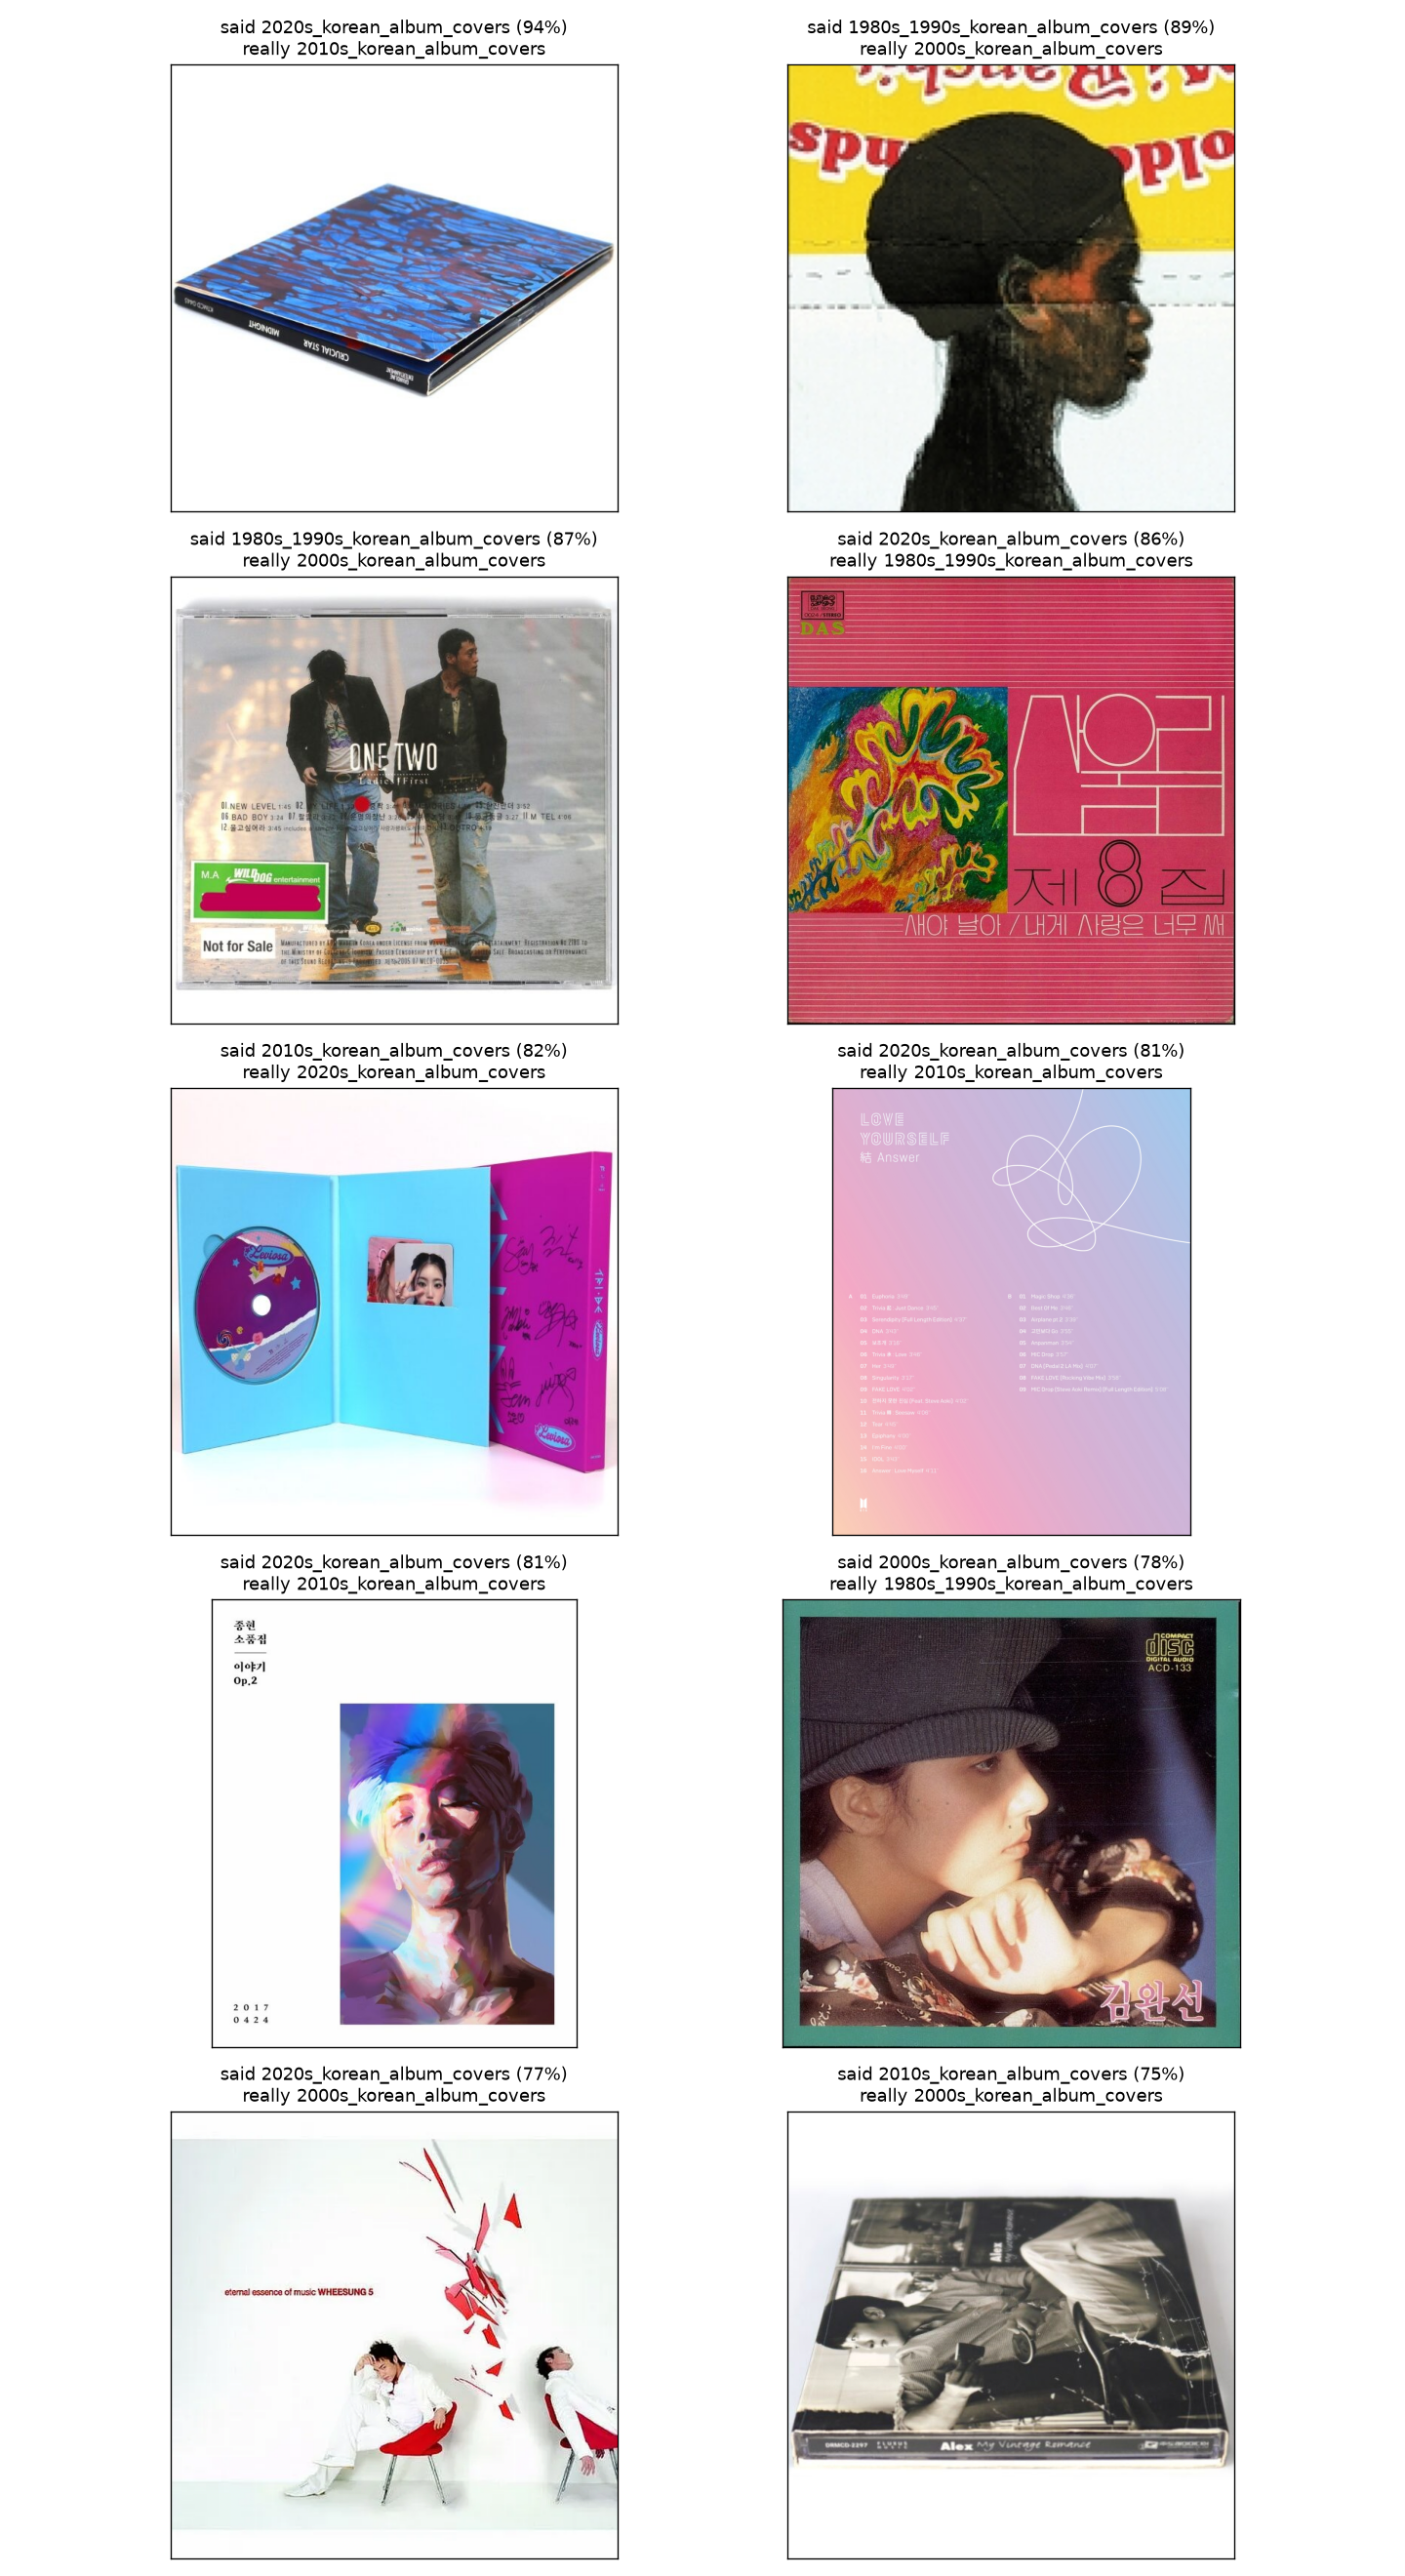
\includegraphics[width=\linewidth,height=0.85\textheight,keepaspectratio]{figures/clean_worst.png}\captionof{figure}{CLEAN's most confident downloaded-test mistakes.}\end{center}
\subsection*{Output of the CLEAN run}
\outputfile{outputs/clean_output.txt}

\section*{Problem 5. Images from a new source}
I manually selected era-appropriate artists and albums from music websites and checked against my downloads. The class counts in Problem 1 meet the minimum of five each. However, I did not preserve site URLs or evidence that the downloader could not have found these sources, so source independence remains unverified.

The saved overlap check compared the 27 new images with 1,682 downloaded images and found no similarity above 0.95; the closest was 0.85. This establishes no detected near copies within that check, not source independence.
\outputfile{outputs/overlap.txt}

The CLEAN accuracies appear side by side in Problem 4: the new-source score is lower than the downloaded-test score. I think source differences and the small evaluation sample may contribute. The new-source confusion matrix is:
\begin{center}
\begin{tabular}{lrrrr}\toprule
Actual $\backslash$ Predicted &1980s--1990s&2000s&2010s&2020s\\\midrule
1980s--1990s&5&1&1&1\\
2000s&1&4&1&0\\
2010s&0&3&2&3\\
2020s&2&0&0&3\\\bottomrule
\end{tabular}
\captionof{table}{CLEAN on new images; rows are actual eras and columns are predictions.}
\end{center}

\subsection*{Five confident mistakes}
These are my interpretations, not isolated causes. Paths below are relative to \path{data/new_images/}; WebP examples were converted to PNG only for report display.
\begin{center}\picturefile[0.4\linewidth]{figures/new_2013.png}\captionof{figure}{\path{2010s_korean_album_covers/2013.webp}: actual 2010s, predicted 2000s (96\%).}\end{center}
I think its monochrome-like aesthetic and freely handwritten-looking English typography resemble 2000s covers. The file itself contains colour.
\begin{center}\picturefile[0.4\linewidth]{figures/new_2012_prime.png}\captionof{figure}{\path{2010s_korean_album_covers/2012'.webp}: actual 2010s, predicted 2020s (89\%).}\end{center}
I think the simple sky background and repeated linear design may look like a polished 2020s layout.
\begin{center}\picturefile[0.32\linewidth]{figures/new_1985.jpg}\captionof{figure}{\path{1980s_1990s_korean_album_covers/1985.jpg}: actual 1980s--1990s, predicted 2000s (87\%).}\end{center}
I could not find a convincing explanation for this mistake. This is not the image with the same filename in Problem 2.
\begin{center}\picturefile[0.4\linewidth]{figures/new_2012.png}\captionof{figure}{\path{2010s_korean_album_covers/2012.webp}: actual 2010s, predicted 2020s (82\%).}\end{center}
I identified this as PSY's Gangnam Style cover. Although the illustration reminds me of its era, I think the vivid colours may have pushed the prediction toward the 2020s.
\begin{center}\picturefile[0.4\linewidth]{figures/new_2014.png}\captionof{figure}{\path{2010s_korean_album_covers/2014.webp}: actual 2010s, predicted 2000s (72\%).}\end{center}
I think its yellowish tone and monochrome-like aesthetic may have contributed to the 2000s prediction; it is not literally grayscale.

\subsection*{How the new images differ}
The downloaded examples include collages on walls, cassette packaging, and angled LP photographs with surrounding cardboard or inserts. CLEAN's test mistakes also include angled packaging and exposed CDs. In contrast, these new examples fill the frame with the cover design, without surrounding desks or packaging.

Physical photographs introduce viewing distance, margins and perspective; those external camera conditions are not identifiable in these digital-cover examples. Their lighting and colour are part of the cover artwork, not a known new photography setup. This comparison describes the inspected examples, not the full distribution. Some new files are WebP, contrary to README's JPEG/PNG instruction, although the saved checker read them successfully.

\section*{Problem 6. The demo}
Address: \url{https://downtownwonn.github.io/mas1004-assignment1-new/}

I confirmed that the demo worked; the saved Problem 7 screenshots show predictions and the model's crop. A green self-test badge and a phone test away from my computer are not documented. The saved checker reports Python--ONNX agreement (largest displayed gap 0.0000); its uncommitted-model warning is from that earlier check, not a verified current deployment diagnosis.

When I uploaded an \emph{agujjim} food photograph, it chose the 2020s; for my close-up portrait photograph, it chose the 2000s, because the classifier has no ``not an album cover'' option. I did not preserve screenshots of these two inputs.

\section*{Problem 7. What the model looks at}
The evidence is the saved web screenshots in \path{results/P5_experiments/}. Every probability vector below uses the order [1980s--1990s, 2000s, 2010s, 2020s], in percent, preserving displayed rounding. The screenshots show the model's crop. Exact requests remain in their original Korean, including typos, as required.

\subsection*{Guess 1. The black circular area resembles an LP}
I thought the black circular area on a 2000s cover might resemble an LP and explain its older-era prediction. I chose to cover it and check whether the older-era probability fell.

My requests to the agent, word for word:
\begin{quote}
“첫번째 사진 가리는거”\\
“회색말고 흰색으로 가려주고, 검은 부분을 더 가려주라”\\
“원형말고 네모낳게 가려주라”
\end{quote}
\sidebyside{figures/p7_1_original.png}{\texttt{1\_original.png}: [90.9, 6.7, 2.2, 0.2]}
{figures/p7_1_modified.png}{\texttt{1\_modified.png}: [51.5, 23.5, 15.9, 9.2]}
\captionof{figure}{Covering the black area with a white rectangle.}
The older era remained the top prediction, but its probability fell. This is consistent with my guess, without confirming it: the rectangle also covers part of the head and face and introduces a white region.

\subsection*{Guess 2. Colour contributes to the 2020s prediction}
My initial colour hypothesis and a confident 2020s mistake led me to remove colour while requesting the same proportions and layout. I then tested the same question on another cover.

My requests to the agent, word for word:
\begin{quote}“자 이번엔 두번째 사진, 원이미지 비율 레이아웃 그대로 유지하면서 무채색으로만 바꿔줘”\end{quote}
\sidebyside{figures/p7_2_original.png}{\texttt{2\_original.png}: [3.8, 5.6, 7.7, 82.9]}
{figures/p7_2_modified.png}{\texttt{2\_modified.png}: [10.5, 28.0, 48.9, 12.6]}
\captionof{figure}{First grayscale change.}
\begin{quote}“이번엔 세번쨰 사진, 원이미지 비율 레이아웃 그대로 유지하면서 무채색으로만 바꿔줘”\end{quote}
\sidebyside{figures/p7_3_original.png}{\texttt{3\_original.png}: [1.0, 1.5, 17.6, 79.9]}
{figures/p7_3_modified.png}{\texttt{3\_modified.png}: [11.1, 3.4, 22.3, 63.1]}
\captionof{figure}{Grayscale change on a second independent original.}
The first prediction changed to the 2010s; the second remained in the 2020s with lower probability. I interpret this as colour-related sensitivity that varies by image, not a rule that grayscale implies an older era. The generative edits may also alter brightness or texture.

\subsection*{Further tests on a misclassified portrait cover}
The original 1980s--1990s portrait cover was classified as 2000s. I explored direction, expression and accessories as possible clues. The following records preserve my changes and observations, but not a specific advance prediction for each change. The front-view, smile and cap-removal comparisons are cumulative, not separate edits of the original.

\subsection*{Change 4. Front-facing portrait}
I changed the direction to see whether the prediction responded.
\begin{quote}“네번쨰 사진, 원이미지 비율 레이아웃 그대로 유지하면서 정면으로만 바꿔줘”\end{quote}
\sidebyside{figures/p7_4_original.png}{\texttt{4\_original.png}: [4.0, 70.1, 0.9, 25.0]}
{figures/p7_4_modified1_front_view.png}{\texttt{4\_modified1\_front\_view.png}: [14.4, 71.3, 6.3, 8.0]}
\captionof{figure}{Front-facing edit.}
The top prediction stayed in the 2000s. The hands and arms also changed, so this was not a direction-only test.

\subsection*{Change 5. Adding a smile}
I added a smile to the front-facing version to explore expression.
\begin{quote}“이번엔 정면 흐뭇하게 웃는 얼굴로 바꿔줘 나머지는 원본 유지하면서”\end{quote}
\sidebyside{figures/p7_4_modified1_front_view.png}{Before smile: [14.4, 71.3, 6.3, 8.0]}
{figures/p7_4_modified2_smile.png}{\texttt{4\_modified2\_smile.png}: [17.2, 66.4, 7.7, 8.7]}
\captionof{figure}{Smile added to the front-facing version.}
The 2000s probability decreased, but the top class did not change.

\subsection*{Change 6. Removing the beret}
I removed the beret from the smiling version to explore the accessory's influence.
\begin{quote}“이번엔 정면에 흐뭇하게 웃는 얼굴에 추가로 베레모를 벗겨줘”\end{quote}
\sidebyside{figures/p7_4_modified2_smile.png}{Before cap removal: [17.2, 66.4, 7.7, 8.7]}
{figures/p7_4_modified3_nocap.png}{\texttt{4\_modified3\_nocap.png}: [27.6, 53.8, 16.6, 2.0]}
\captionof{figure}{Beret removed from the smiling version.}
The 2000s probability decreased and the older-era probability increased. Removing the cap also generated previously hidden hair, so I cannot isolate the cap's effect.

\subsection*{Additional observation. Fuller wavy hair}
\sidebyside{figures/p7_4_modified3_nocap.png}{Capless comparison: [27.6, 53.8, 16.6, 2.0]}
{figures/p7_4_modified4_hair.png}{\texttt{4\_modified4\_hair.png}: [8.5, 66.7, 21.7, 3.1]}
\captionof{figure}{Preserved fuller, wavy-hair version.}
The saved version has fuller wavy hair, but my exact request is unavailable. I include the evidence without treating it as a fully documented independent test.

\subsection*{Change 7. Metal-framed glasses}
I requested glasses twice; only one confirmed result screenshot remains.
\begin{quote}
“이번엔 금속테 안경을 씌워줘”\\
“이번엔 금속테 안경을 씌워줘”
\end{quote}
\sidebyside{figures/p7_4_modified3_nocap.png}{Visually corresponding capless version: [27.6, 53.8, 16.6, 2.0]}
{figures/p7_4_modified5_glasses.png}{\texttt{4\_modified5\_glasses.png}: [41.4, 46.1, 10.5, 1.9]}
\captionof{figure}{Glasses version and its visually corresponding comparison.}
Relative to this comparison, the 2000s probability fell and the older-era probability rose. The hair resembles the capless version rather than the wavy-hair edit. I cannot confirm the actual input file or which request produced the result, so I do not treat these files as one linear sequence or two glasses tests.

\subsection*{Change 8. Enlarging the singer's name}
I expected a more prominent singer's name might help the model recognize the older era. I requested:
\begin{quote}“이번엔 우측하단 김완선 글자를 두배크기로 키워줘”\end{quote}
\sidebyside{figures/p7_4_modified5_glasses.png}{Visually corresponding glasses version: [41.4, 46.1, 10.5, 1.9]}
{figures/p7_4_modified6_bigletter.png}{\texttt{4\_modified6\_bigletter.png}: [4.0, 22.9, 36.8, 36.3]}
\captionof{figure}{Enlarged-name version and its visually corresponding comparison.}
Contrary to my expectation, the older-era probability fell and the 2010s became the top class, narrowly ahead of the 2020s. The actual edit input is not documented; this does not show that the model read the name or that text size alone caused the change. ``Twice'' describes my request, not a measured output size.

\subsection*{What I now think the model uses}
I tentatively think colour, layout, portrait direction, expression and accessories can influence predictions. My strongest observation is that the selected covers are sensitive to edits; I have not identified a feature that determines the release era. Generative changes and cumulative baselines limit causal interpretation.

Only grayscale was tested on two independent originals. I did not document several independent originals for each other change, all advance hypotheses and expected directions, the hair request, or the exact glasses/text input chain. These are remaining gaps against Problem 7, not additional completed tests.

\clearpage
\section*{Appendix. Output of check.py}
This is the complete saved four-class check, without rerunning evaluation or deleting its historical warning.
\outputfile{outputs/check.txt}

\section*{Supporting evidence}
Saved outputs below retain their original text, language and warnings. Only report copies of UTF-16 logs were converted to UTF-8. The exact Korean P7 requests and untranslated evidence are the exceptions to the report's English prose.
\subsection*{Saved model and dataset consistency inspection}
\outputfile{outputs/step13_inspection.txt}
\subsection*{Accuracy differences calculated from final printed values}
\outputfile{outputs/accuracy_gaps.txt}
\subsection*{Asset and preprocessing audit}
\outputfile{outputs/asset_audit.txt}

\section*{README requirement check}
This checklist maps all 25 ``Write this down'' items to the report. ``Partial'' identifies missing evidence, not a completed requirement.
\begin{enumerate}
\item \textbf{P1: Category choice and interest.} Problem 1, ``Why these categories.''
\item \textbf{P1: Expected features before training.} Problem 1, ``What I expected the model to use.''
\item \textbf{P1: Class counts.} Problem 1 table and saved run outputs.
\item \textbf{P2: Original/prepared pair and crop loss --- partial.} Problem 2 figure and description show edge and lettering loss; no specific important-subject loss example is documented.
\item \textbf{P3: Loss curves and trends.} Problem 3 loss table, all run curves, and CLEAN curves in Problem 4.
\item \textbf{P3: Train--test gap and meaning.} Problem 3 gap discussion and supporting calculation output.
\item \textbf{P3: Confusion matrix and surprise.} Problem 3 matrices and my expectation; CLEAN matrix in Problem 4.
\item \textbf{P3: ImageNet versus random initialization.} Problem 3 comparison and complete run outputs; proposed reasons are interpretations.
\item \textbf{P3: Last-layer versus full training.} Problem 3 comparison, including the different learning rate.
\item \textbf{P4: Rule before cleaning.} Problem 4, ``My rule,'' with later era-mismatch additions distinguished.
\item \textbf{P4: Three kinds of junk.} Problem 4 includes a picture and recorded removal reason for each.
\item \textbf{P4: Removals by class and reason.} Problem 4 cumulative table and saved early count output; unlogged actions remain outside the table.
\item \textbf{P4: Near copies and decisions --- partial.} Problem 4 distinguishes pairs, exact-duplicate groups and files; complete pair-level decisions are missing.
\item \textbf{P4: Top-20 removals and missed junk --- partial.} Problem 4 records 7/12/8/9 cumulative logged removals; specific junk missed by my first review or by the list is undocumented.
\item \textbf{P4: Before/after accuracy.} Problem 4 side-by-side table and complete comparison output; changed splits and supplementation are disclosed.
\item \textbf{P5: Source independence and overlap --- partial.} Problem 5 includes my sourcing account and complete overlap output; site URLs and evidence of search-inaccessible sources are missing.
\item \textbf{P5: Downloaded-test/new-source accuracy side by side.} Problem 4 comparison table, referenced in Problem 5, and full checker output.
\item \textbf{P5: Five confident mistakes and explanations.} Problem 5 includes each picture, path, label and probability, with my interpretations; I could not explain the 1985 mistake.
\item \textbf{P5: Background, lighting, angle, distance and surroundings.} Problem 5 compares inspected examples and identifies unknown camera conditions.
\item \textbf{P6: Demo address.} Problem 6 supplies the URL. Required green-badge and away-from-computer phone checks remain undocumented.
\item \textbf{P6: Out-of-category input.} Problem 6 records my food and portrait observations; screenshots were not preserved.
\item \textbf{P7: Guesses and their motivation --- partial.} Problem 7 records my LP, colour and name-size expectations and portrait tests; some advance hypotheses are missing.
\item \textbf{P7: Changes, rationale, paired images and answers --- partial.} Problem 7 preserves every comparison and probability vector. Exact glasses/text baselines and several independent originals per change are not documented.
\item \textbf{P7: Exact requests --- partial.} All supplied requests and both glasses calls are preserved verbatim; the hair-edit request is unavailable.
\item \textbf{P7: Current interpretation and confidence.} Problem 7 closes with my tentative interpretation and the limits of the tests.
\end{enumerate}
\textbf{Other checks:} The report retains the four pre-cleaning runs, the CLEAN run, all previously referenced figures and saved outputs, and the complete four-class checker. Some new-source files are WebP rather than the required JPEG/PNG. My name and student ID still need to be filled in.
\end{document}